\documentclass{article}

\usepackage[utf8]{inputenc}
\usepackage{graphicx}
\usepackage{natbib}
\usepackage{amsmath}
\usepackage{amssymb}
\usepackage{amsthm}
\usepackage{mathpartir}
\usepackage{bm}
\usepackage{hyperref}
\usepackage{cleveref}
%\usepackage{draftwatermark}

\newtheorem{lemma}{Lemma}
\newtheorem{theorem}{Theorem}
\newtheorem{corollary}{Corollary}

%\SetWatermarkText{Draft}
%\SetWatermarkScale{5}
%\SetWatermarkColor[gray]{0.90}

\newcommand{\Pend}{\bm{0}}
\newcommand{\Ppar}[2]{#1 \mid #2}
\newcommand{\Pres}[2]{(\bm{\nu} #1)~#2}
\newcommand{\Pout}[3]{#1 ! #2 . #3}
\newcommand{\Pin}[3]{#1 ? (#2) . #3}
\newcommand{\Pchoice}[2]{#1 + #2}
\newcommand{\Preplicate}[1]{{!}#1}

\newcommand{\freenames}[1]{\textrm{fn}(#1)}
\newcommand{\boundnames}[1]{\textrm{bn}(#1)}
\newcommand{\names}[1]{\textrm{n}(#1)}

\newcommand{\freevars}[1]{\textrm{fv}(#1)}
\newcommand{\boundvars}[1]{\textrm{bv}(#1)}
\newcommand{\vars}[1]{\textrm{vars}(#1)}

\newcommand{\alphacon}[2]{#1 =_{\alpha} #2}
\newcommand{\subst}[3]{#1\{#2/#3\}}

\newcommand{\Aoutf}[2]{#1 ! #2}
\newcommand{\Aoutb}[2]{#1 ! (#2)}
\newcommand{\Ain}[2]{#1 ? #2}
\newcommand{\Atau}{\tau}

\newcommand{\transition}[3]{#1 \xrightarrow{#2} #3}

\newcommand{\observable}[2]{#1\downarrow_{#2}}
\newcommand{\obsin}[1]{#1?}
\newcommand{\obsout}[1]{#1!}

\newcommand\sbullet[1][.5]{\mathbin{\hbox{\scalebox{#1}{$\bullet$}}}}
\newcommand{\sbbisim}[2]{#1 \overset{\sbullet}{\sim} #2}
\newcommand{\nsbbisim}[2]{#1 \not\overset{\sbullet}{\sim} #2}

\newcommand{\ctxhole}{[\cdot]}
\newcommand{\applyctx}[2]{#1[#2]}
\newcommand{\sbcong}[2]{#1 \simeq^c #2}

\newcommand{\applysubst}[2]{#2#1}

\newcommand{\Presd}[3]{(\bm{\nu} #1#2)~#3}
\newcommand{\scong}[2]{#1 \equiv #2}

\newcommand{\reduces}[2]{#1 \rightarrow #2}

\newcommand{\Tend}{\mathbf{end}}
\newcommand{\Tbase}{\mathbf{base}}
\newcommand{\Tin}[1]{{?}.#1}
\newcommand{\Tout}[1]{{!}.#1}

\newcommand{\hastype}[2]{#1 : #2}

\newcommand{\un}[1]{\mathbf{un}(#1)}
\newcommand{\lin}[1]{\mathbf{lin}(#1)}

\newcommand{\Cempty}{\varnothing}
\newcommand{\Cadd}[2]{#1, #2}
\newcommand{\Csplit}[2]{#1 \circ #2}
\newcommand{\Cupdate}[2]{#1 + #2}

\newcommand{\dual}[1]{\overline{#1}}

\newcommand{\types}[2]{#1 \vdash #2}

%% Local Variables:
%% mode: latex
%% TeX-master: "main"
%% End:


\begin{document}

\title{POPLMark goes Concurrent!\\Challenge problems for process calculi and behavioural types}

\maketitle

\begin{abstract}
  The publication of POPLMark spearheaded the era of publishing formal
  proofs alongside with new research. This fostered an era of
  high-quality and high-assurance proofs at top venues for programming
  language research. This paper simultaneously acknowledges the impact
  of the original POPLMark challenge, and proposes a new benchmark
  intended to stimulate the research and dissemination of techniques
  that address the particular challenges of process calculi and
  behavioural type systems. In this work we propose three challenge
  problems concerning to process calculi and name passing, linearity
  in behavioural type systems, and coinductive reasoning for process
  algebras.
\end{abstract}

\section{Introduction}

In recent years, the programming language community has embraced
machine checked proofs for theoretical results in papers. The
POPLMark~\cite{POPLMark} challenge was proposed for this purpose,
and to get the community on track. Since then the number of formal
proofs accompanying papers has grown\footnote{add some POPL/PLDI/etc
  statistics here}. However, formal proofs are not equally spread in
the field. In this call to action, we propose to extend the key
contribution of challenges like POPLMark is to help develop the
necessary momentum and culture to be able to formalise results to the
concurrent calculi community by proposing a challenge the exercises
the key aspects of reasoning about process calculi. We propose this
document, and a \href{https://concurrentbenchmark.github.io/}{website}
to enable the community to collaborate on the project.

It has been a long time since the original challenge, and many changes
have happened. Particularly, POPLMark and any challenge cannot address
every conceivable technique. Challenges have to be simple so that the
techniques are not shadowed by technical details and also feasible to
implement without heroic efforts. In that vein, it is apparent that
new challenges are needed, work like POPLMark
Reloaded~\cite{POPLMarkReloaded} strives to extend the scope of the
original challenge to proofs using logical relations. This technique
is crucial to many current developments.

As mentioned before, in this work we address another expansion of
scope for such challenges, going from the $\lambda$-calculus to
process calculi such as the $\pi$-calculus and session type systems
(and other behavioural type systems). These systems require particular
insights to implement. So far, we have identified three key
aspects\footnote{We want to keep the number low, but the exact nature
  of the challenges is still open to discussion (as are most things in
  this project).}. First, the idea of scope extrusion in name passing
calculi. This generalises the idea of binders in ways that techniques
that were adequate for $\lambda$-calculus binders are not so
convenient for name passing systems. Second, session types in
particular, and behavioural types in general often depend on linearity
in their type systems. The formalisation of linear type systems posses
a challenge given that it is not uniformly well supported among the
many proof assistants. Finally, processes in concurrent systems often
contain infinite behaviour that is typically modelled with
coinduction. This technique is used to reason about (bi)similarity
between processes, the equivalence of their traces, or subtyping
between infinite trees of possible behaviours. This challenge
concentrates on those issues.

In this work we propose a challenge where each part independently
exercises one of the three areas, however it is often the case that a
problem requires more than one of these techniques simultaneously. In
this work, we explore them in isolation, in order to facilitate the
implementation of smaller solutions. Concretely, we do not address the
idea of how to combine these techniques, leaving the discussion of
that to the future when we have collected enough entries to these
problems.

We do not claim in this work that these problems have never been
approached and formalised before. In fact, the contrary is true. All
of these problems have been addressed in several forms. This motivates
this challenge to enable an easier comparison between solutions (since
they all implement the same challenge), and in a setting that is
\emph{simple enough to not be distracting, yet complex enough that we can
compare strengths and weaknesses of each}.

The rest of this paper is structured in the following way:
\cref{sec:rationale} expands on the rationale for the selected
challenge problems. Then \cref{sec:problems} presents the problems. We
discuss the solutions in \cref{sec:solutions}, in particular
\cref{sec:tutorial} walks through a tutorial solution. And finally
\cref{sec:conclusion} presents some conclusions and it contains a call
to action to invite the submission of new solutions.

\section{Rationale for choosing the problems}\label{sec:rationale}

 The idea is to explore three areas: scope
extrusion in name passing calculi, linearity requirements in
behavioural types, and finally coinductive reasoning in trace
equivalence, (bi)similarity, or subtyping in the presence of
recursion.

The idea is to have three small problems in the aforementioned
subjects that are independent of each other and that are easy to
understand and to implement. This is important so we have more
entries. They have to be small so it is not a lot to read, and
independent so people may choose to implement only one of them, or
work on them in any order. Moreover, the specification should only
need to be met in spirit. The idea is to provide a solution author
with some space to show the best aspects of their solution even if
that means adapting the problem definition while keeping the spirit of
the challenge.

Finally, it will be important to mention in the rationale for problems that
the key aspects are:
\begin{itemize}
\item Scope extrusion
\item Linearity
\item Coinduction
\end{itemize}

But the exact presentation of the concrete problems is somewhat
flexible. In the sense that the use of certain techniques or tools may
require changing the presentation of the system to fit the technique.
We are more interested in the techniques that are applicable to these
problems as a class of problems than to the exact specification we
propose. Of course, for clarity if a solution changes the definition
it should document in what sense the definition differs. So changes
allowed, and even encouraged, but the result should be ``morally'' the
same system and there should be a rationale for the changes in
presentation. That way we not only see valid techniques but also what
presentation of the rules to use and the rationale to chose a
particular approach.

\section{The challenge problems} \label{sec:problems}

\begin{figure}[h]
  \centering
  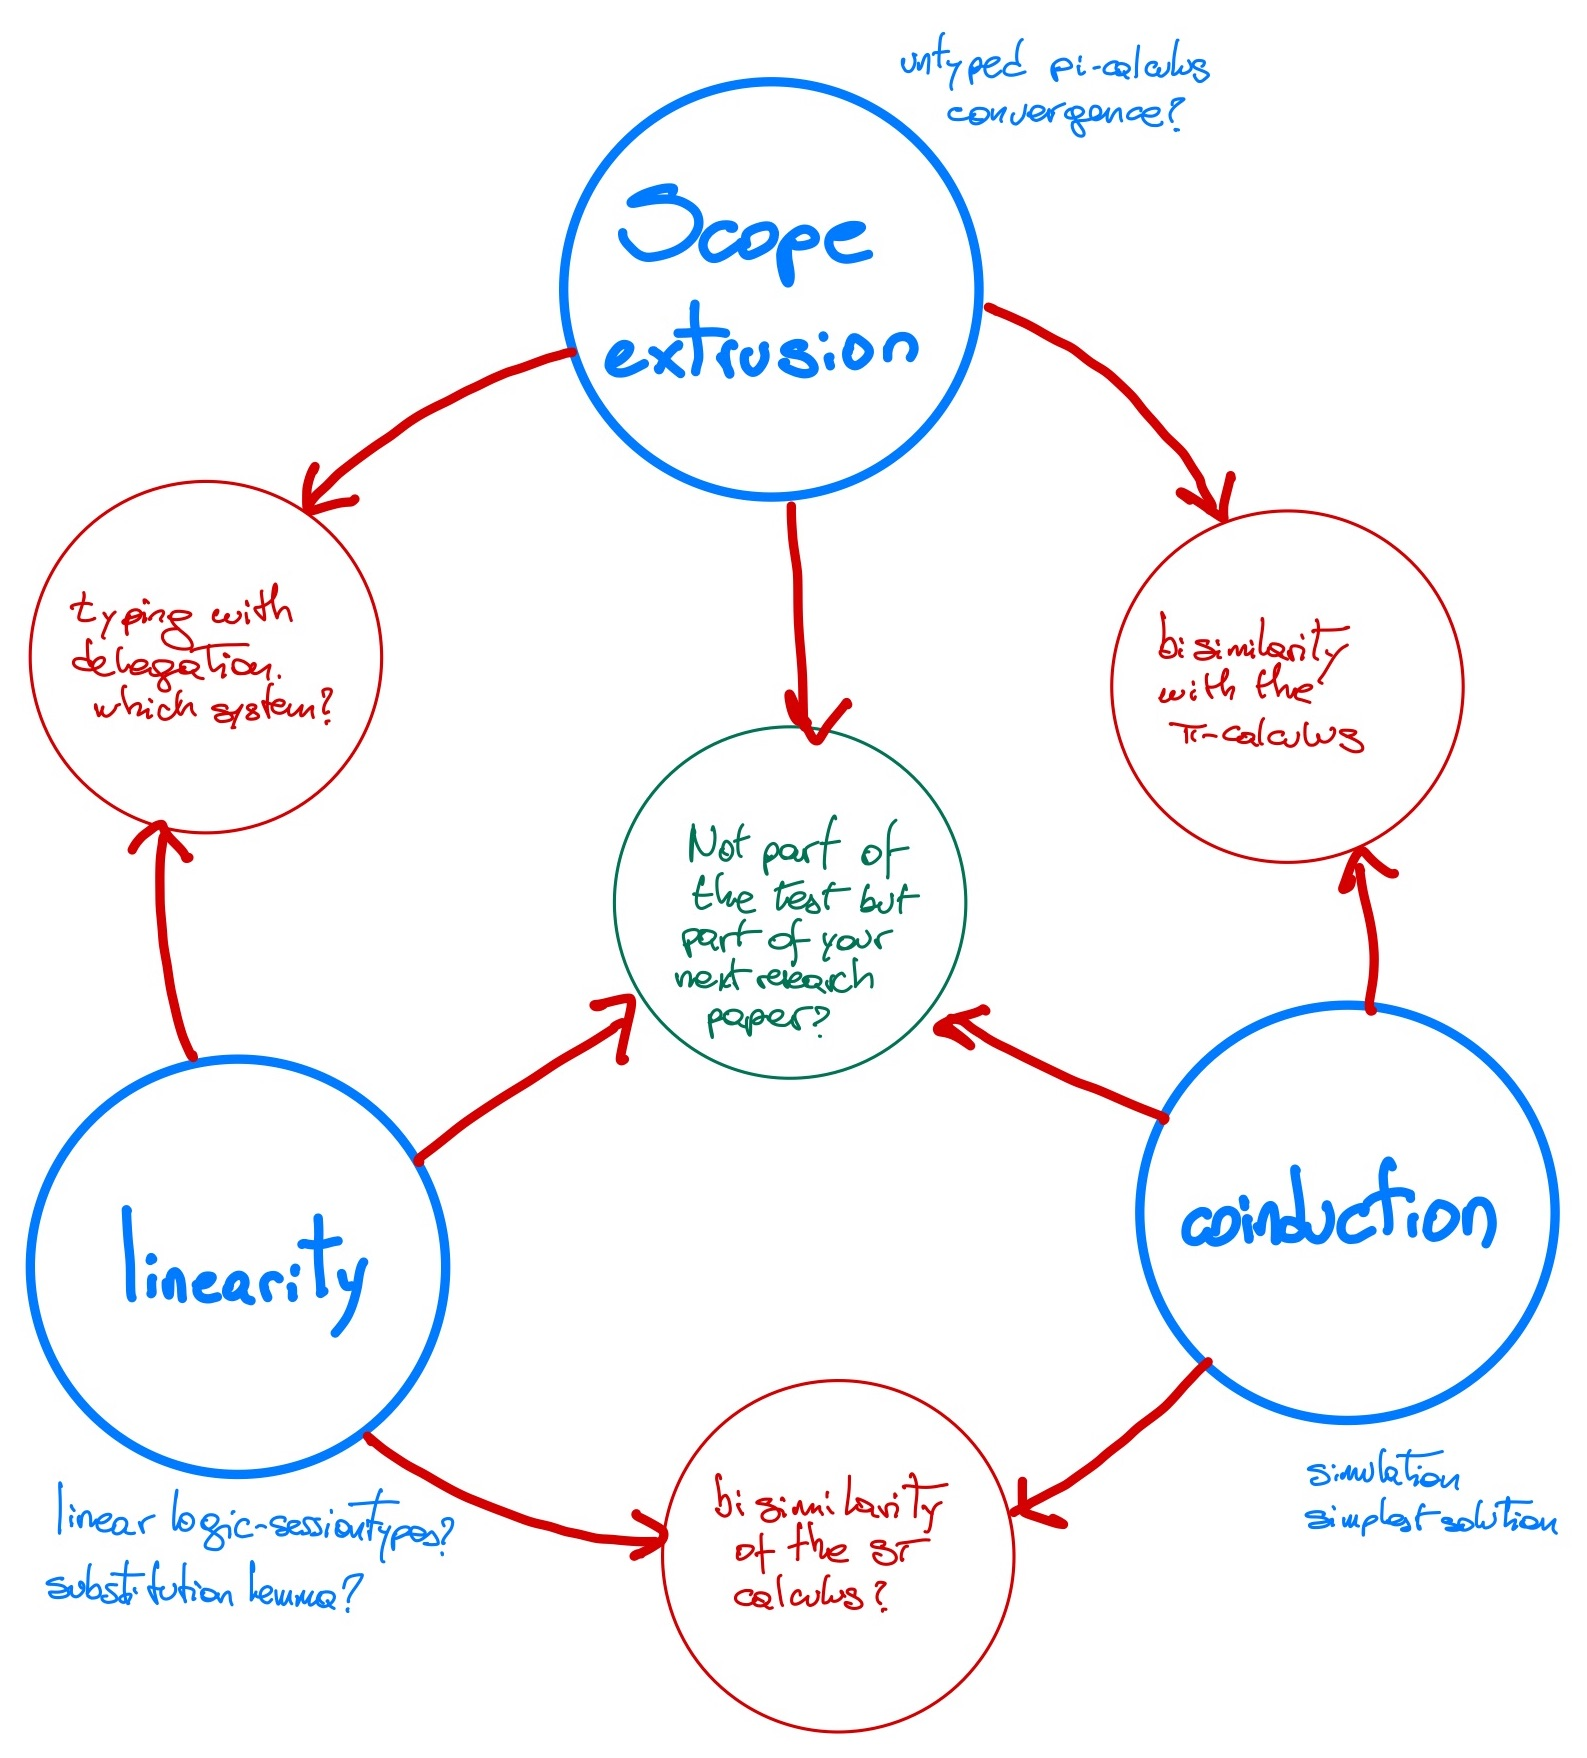
\includegraphics[width=0.75\textwidth]{../images/benchmark.jpeg}
  \caption{The benchmark's big picture.}
  \label{fig:bigpic}
\end{figure}

The big picture for the benchmark can be seen in \cref{fig:bigpic}
where the three pillars (i.e.: concepts typically needed for process
calculus proofs) appear in blue, with some ideas of what to prove. And
a second step of combining the three aspects (for a total of six steps
for the whole benchmark), and of course the $+1$-step for the
combination of everything on the reader's next research papers.

\documentclass[a4paper]{article}

\usepackage{amsmath}
\usepackage{amssymb}
\usepackage{amsthm}
\usepackage[utf8]{inputenc}
\usepackage{mathpartir}
\usepackage{bm}
\usepackage{graphicx}

\newtheorem{lemma}{Lemma}
\newtheorem{theorem}{Theorem}

\newcommand{\Pend}{\bm{0}}
\newcommand{\Ppar}[2]{#1 \mid #2}
\newcommand{\Pres}[2]{(\bm{\nu} #1)~#2}
\newcommand{\Pout}[3]{#1 ! #2 . #3}
\newcommand{\Pin}[3]{#1 ? (#2) . #3}
\newcommand{\Pchoice}[2]{#1 + #2}
\newcommand{\Preplicate}[1]{{!}#1}

\newcommand{\freenames}[1]{\textrm{fn}(#1)}
\newcommand{\boundnames}[1]{\textrm{bn}(#1)}
\newcommand{\names}[1]{\textrm{n}(#1)}

\newcommand{\alphacon}[2]{#1 =_{\alpha} #2}
\newcommand{\subst}[3]{#1\{#2/#3\}}

\newcommand{\Aoutf}[2]{#1 ! #2}
\newcommand{\Aoutb}[2]{#1 ! (#2)}
\newcommand{\Ain}[2]{#1 ? #2}
\newcommand{\Atau}{\tau}

\newcommand{\transition}[3]{#1 \xrightarrow{#2} #3}

\newcommand{\observable}[2]{#1\downarrow_{#2}}
\newcommand{\obsin}[1]{#1?}
\newcommand{\obsout}[1]{#1!}

\newcommand\sbullet[1][.5]{\mathbin{\hbox{\scalebox{#1}{$\bullet$}}}}
\newcommand{\sbbisim}[2]{#1 \overset{\sbullet}{\sim} #2}

\begin{document}

\section{Challenge: Scope Extrusion}
The idea of this challenge is to formalize a proof that requires scope extrusion.
Scope extrusion is the notion that a process can send restricted names to another process, as long as the restriction can safely be ``extruded'' (i.e.\ expanded) to include the recieving process.
This e.g.\ allows a process to set up a private connection by sending a restricted name to another process, then using this name for further communication.

The setting for this challenge is an untyped \( \pi \)-calculus, the syntax and semantics of which are presented below.
The objective of this challenge is to prove that barbed bisimulation for this calculus is an equivalence relation.

\subsection{Syntax}
We assume the existence of some type of \emph{names}, values of which we will denote by \( x, y, \dots \).
The syntax is then:
\begin{align*}
  P,Q :=&&& \Pend \\
  |&&& \Pout{x}{y}{P} \\
  |&&& \Pin{x}{y}{P} \\
  |&&& \Ppar{P}{Q} \\
  |&&& \Pres{x}{P} \\
  |&&& \Pchoice{P}{Q}
\end{align*}
The process \( \Pend \) is \emph{inaction}: a process which can do nothing.
The process \( \Pout{x}{y}{P} \) is an \emph{output}, which can send the name \( y \) via \( x \), then continue as \( P \).
The process \( \Pin{x}{y}{P} \) is an \emph{input}, which can receive a name via \( x \), then continue as \( P \) with the received name substituted for \( y \).
The input operator thus binds the name \( y \) in \( P \).
The process \( \Ppar{P}{Q} \) is the \emph{composition} of process \( P \) and process \( Q \).
The two components can proceed independently of each other, or they can interact via shared names.
The process \( \Pres{x}{P} \) is the \emph{restriction} of the name \( x \) to \( P \).
Components in \( P \) can use the name \( x \) to interact with each other, but not with processes outside of the restriction.
The restriction operator thus binds the name \( x \) in \( P \).
Note that the scope of a restriction may change when processes interact.
The process \( \Pchoice{P}{Q} \) is a non-deterministic \emph{choice} between continuing as the process \( P \) or as the process \( Q \).
Note that there is no recursion or replication in the syntax, and thus no infinite behaviours can be expressed.

We will use the notation \( \freenames{P} \) to denote the set of names that occur free (i.e.\ not bound by a restriction or an input) in \( P \).
We will use the notation \( \boundnames{P} \) to denote the set of names that occur bound (by a restriction or an input) in \( P \).
We will use the notation \( \subst{P}{x}{y} \) to denote the process \( P \) with \( x \) substituted for \( y \).

Two processes \( P \) and \( Q \) are \( \alpha \)-convertible, written \( \alphacon{P}{Q} \), if \( Q \) can be obtained from \( P \) by a finite number of substitutions of bound names.
As a convention, we will identify \( \alpha \)-convertible processes.

As a convention, we assume that the bound names occurring in any collection of processes are chosen to be different from the free names occurring in those processes and from the names occurring in any substitutions applied to the processes.
This is justified because any overlapping names may be \( \alpha \)-converted such that the assumption is satisfied.

\subsection{Semantics}
The semantics of the system describe the actions that the system can perform by defining a labelled transition relation on processes.
The transitions are labelled by \emph{actions}, the syntax of which are as follows:
\begin{align*}
  \alpha := &&& \Aoutf{x}{y} \\
  |&&& \Ain{x}{y} \\
  |&&& \Aoutb{x}{y} \\
  |&&& \Atau
\end{align*}
The \emph{free output action} \( \Aoutf{x}{y} \) is sending the name \( y \) via \( x \).
The \emph{input action} \( \Ain{x}{y} \) is receiving the name \( y \) via \( x \).
The \emph{bound output action} \( \Aoutb{x}{y} \) is sending a fresh name \( y \) via \( x \).
The \emph{internal action} \( \Atau \) is performing some unobservable action, e.g.\ internal communication.

We will again use the notation \( \freenames{\alpha} \) to denote the set of names that occur free in the action \( \alpha \) and the notation \( \boundnames{\alpha} \) to denote the set of names that occur bound in the action \( \alpha \).
In the free output action \( \Aoutf{x}{y} \) and the input action \( \Ain{x}{y} \), both \( x \) and \( y \) are free names.
In the bound output action \( \Aoutb{x}{y} \), \( x \) is a free name, while \( y \) is a bound name.
We will further use the notation \( \names{\alpha} \) to denote the union of \( \freenames{\alpha} \) and \( \boundnames{\alpha} \), i.e.\ the set of all names that occur in the action \( \alpha \).

The transition relation is then defined by the following rules:
\begin{mathpar}
  \inferrule[Out]{ }{\transition{\Pout{x}{y}{P}}{\Aoutf{x}{y}}{P}}
  \and
  \inferrule[In]{ }{\transition{\Pin{x}{z}{P}}{\Ain{x}{y}}{\subst{P}{y}{z}}}
  \and
  \inferrule[Sum-L]{\transition{P}{\alpha}{P'}}{\transition{\Pchoice{P}{Q}}{\alpha}{P'}}
  \and
  \inferrule[Sum-R]{\transition{P}{\alpha}{P'}}{\transition{\Pchoice{Q}{P}}{\alpha}{P'}}
  \and
  \inferrule[Par-L]{\transition{P}{\alpha}{P'} \\ \boundnames{\alpha} \cap \freenames{Q} = \emptyset}{\transition{\Ppar{P}{Q}}{\alpha}{\Ppar{P'}{Q}}}
  \and
  \inferrule[Par-R]{\transition{Q}{\alpha}{Q'} \\ \boundnames{\alpha} \cap \freenames{P} = \emptyset}{\transition{\Ppar{P}{Q}}{\alpha}{\Ppar{P}{Q'}}}
  \and
  \inferrule[Comm-L]{\transition{P}{\Aoutf{x}{y}}{P'} \\ \transition{Q}{\Ain{x}{y}}{Q'}}{\transition{\Ppar{P}{Q}}{\Atau}{\Ppar{P'}{Q'}}}
  \and
  \inferrule[Comm-R]{\transition{P}{\Ain{x}{y}}{P'} \\ \transition{Q}{\Aoutf{x}{y}}{Q'}}{\transition{\Ppar{P}{Q}}{\Atau}{\Ppar{P'}{Q'}}}
  \and
  \inferrule[Close-L]{\transition{P}{\Aoutb{x}{z}}{P'} \\ \transition{Q}{\Ain{x}{z}}{Q'} \\ z \notin \freenames{Q}}{\transition{\Ppar{P}{Q}}{\tau}{\Pres{z}{\Ppar{P'}{Q'}}}}
  \and
  \inferrule[Open]{\transition{P}{\Aoutf{x}{z}}{P'} \\ z \neq x}{\transition{\Pres{z}{P}}{\Aoutb{x}{z}}{P'}}
  \and
  \inferrule[Close-R]{\transition{P}{\Ain{x}{z}}{P'} \\ \transition{Q}{\Aoutb{x}{z}}{Q'} \\ z \notin \freenames{P}}{\transition{\Ppar{P}{Q}}{\tau}{\Pres{z}{\Ppar{P'}{Q'}}}}
  \and
  \inferrule[Res]{\transition{P}{\alpha}{P'} \\ z \notin \names{\alpha}}{\transition{\Pres{z}{P}}{\alpha}{\Pres{z}{P'}}}
\end{mathpar}
Note that there is no rule for inferring transitions from \( \Pend \), and that there is no rule for inferring an action of an input or output process except those that match the input/output capability.
Note also that due to rule \TirName{In}, the process \( \Pin{x}{z}{P} \) can receive \emph{any} name.

As a convention, we assume that bound names of any processes or actions are chosen to be different from the names that occur free in any other entities under consideration, such as processes, actions, substitutions, and sets of names.
The convention has one exception, namely that in the transition \( \transition{P}{\Aoutb{x}{z}}{Q} \), the name \( z \) (which occurs bound in \( P \) and the action \( \Aoutb{x}{z} \)) may occur free in \( Q \).
Without this exception it would be impossible to express scope extrusion.

\subsection{Bisimilarity}
Our notion of process equivalence relations builds on a notion of \emph{observables}.
If we allow ourselves only to observe internal transitions, we will relate either too few processes (in the strong case where we relate only processes with exactly the same number of internal transitions) or every process (in the weak case where we relate processes with any amount of internal transitions).
We must therefore allow ourselves to observe more, and here choose to define the observables of a process as the names it can use for sending and receiving.

To this end, we define the \emph{observability predicate} \( \observable{P}{\mu} \) by the following rules:
\begin{align}
  \observable{P}{\obsin{x}}  &\quad \textrm{if \( P \) can perform an input action via \( x \).} \\
  \observable{P}{\obsout{x}} &\quad \textrm{if \( P \) can perform an output action via \( x \).}
\end{align}

Two processes \( P \) and \( Q \) are then \emph{strongly barbed bisimilar}, written \( \sbbisim{P}{Q} \), if:
\begin{gather}
  \observable{P}{\mu}~\textrm{implies}~\observable{Q}{\mu} \\
  \transition{P}{\Atau}{P'}~\textrm{implies}~\transition{Q}{\Atau}{Q'}~\textrm{for some \( Q' \) with}~\sbbisim{P'}{Q'} \\
  \observable{Q}{\mu}~\textrm{implies}~\observable{P}{\mu} \\
  \transition{Q}{\Atau}{Q'}~\textrm{implies}~\transition{P}{\Atau}{P'}~\textrm{for some \( P' \) with}~\sbbisim{P'}{Q'}
\end{gather}
Note that, since our calculus does not have infinite behaviour, we do not specify that the relation is the largest of its kind, and the relation is thus not coinductively defined.

\subsection{Challenge}
The objective of this challenge is to prove the following theorem:
\begin{theorem}
  \( \sbbisim{}{} \) is an equivalence relation, that is, the relation is reflexive, symmetric, and transitive.
\end{theorem}

\section{Challenge: Coinduction}
The idea of this challenge is to formalize a proof that requires coinductive techniques.
Coinduction is a proof technique for infinite structures, which arise in this context due to systems with behaviours that continue indefinitely.
Coinduction is the dual of induction: whereas induction is useful for proving properties of least fixed points, coinduction is useful for proving properties of greatest fixed points.

The setting for this challenge is an untyped calculus of communicating systems with replication of processes, the syntax and semantics of which are presented below.
The objective of this challenge is to prove that strong barbed bisimulation for this calculus is an equivalence relation.

\section{Challenge: Linearity}
The setting for this challenge is a restricted \( \pi \)-calculus with a session type system.

The objective of this challenge is to prove type preservation.

\section{Bonus challenges}

\subsection{Linearity and Scope Extrusion}
The setting for this challenge is the \( \pi \)-calculus with a session type system.

The objective of this challenge is to prove type preservation.

\subsection{Scope Extrusion and Coinduction}
The setting for this challenge is a simply typed \( \pi \)-calculus.

The objective of this challenge is to prove bisimulation.

\subsection{Coinduction and Linearity}
The setting for this challenge is the Calculus of Communicating Systems with a session type system.

The objective of this challenge is to prove type preservation.

\section{Future work}
\begin{itemize}
\item Multiparty session types
\item Choreography
\item Encodings
\item Code extraction
\end{itemize}

\end{document}

\section{The solutions}\label{sec:solutions}

\subsection{A tutorial solution on paper}\label{sec:tutorial}

Probably the skeleton here and more details on an appendix.

\subsection{Flexibility in solving a challenge}

\dots

% \readfiletrue
% \myfile{../appst}

\section{Future work}
\begin{itemize}
\item Multiparty session types
\item Choreography
\item Encodings
\item Code extraction
\item Conversation types
\item Psi-calculus
\item Model checking for system properties
\item More general types than session types
\end{itemize}

\section{Conclusion and related work} \label{sec:conclusion}

\bibliographystyle{plainnat}
\bibliography{../references}

\label{lastpage01}

\end{document}
